\documentclass[11pt]{article}
\usepackage[margin=1in]{geometry}
\usepackage[T1]{fontenc}
\usepackage{lmodern}
\usepackage{amsmath,amssymb,amsthm}
\usepackage{graphicx}
\usepackage{xcolor}
\usepackage{microtype}
\usepackage[hidelinks]{hyperref}

\newtheorem{theorem}{Theorem}
\newtheorem{lemma}[theorem]{Lemma}
\newcommand{\RR}{\mathbb R}
\newcommand{\Detw}{\operatorname{Det}\mathcal D^2}
\newcommand{\MA}{\operatorname{MA}}

\title{A Literature-Implied Arbitrary-Domain Subcase for\\
Very Weak Monge--Amp\`ere Rigidity in arXiv:2206.09224}
\author{Run fa\_banach\_001, agent\_lane\_05}
\date{13 August 2026}

\begin{document}
\maketitle

\section*{Status and source problem}

This is a \texttt{literature\_implied\_answer (partial subcase)} packet.
Pakzad proves the full-plane rigidity theorem for
$C^{1,\alpha}$ very weak Monge--Amp\`ere solutions when $\alpha>2/3$, but
Remark~1.6 on PDF page~5 records that the analogous result on an arbitrary
domain remains open \cite{Pakzad}.

\begin{center}

\includegraphics[width=.96\textwidth]{figures/open_problem_crop.png}
\end{center}

The extra hypothesis below isolates the missing topological issue: gradient
fibers.  Under local injectivity, the desired conclusion follows by combining
Pakzad's regular-point degree argument with Ball's strict-convexity theorem,
in the exact form restated by Guerra and Tione \cite[Corollary~5.2]{GT}.

\section*{Partial answer}

For $v\in C^1(\Omega)$ and $x\in\Omega$, write
\[
 v_x(z)=v(z)-v(x)-\langle \nabla v(x),z-x\rangle.
\]

\begin{theorem}[Locally injective-gradient subcase]\label{thm:main}
Let $\Omega\subset\RR^2$ be a connected open set, let
$2/3<\alpha<1$, and let $v\in C^{1,\alpha}_{\mathrm{loc}}(\Omega)$ satisfy
\[
 \Detw v=f\geq0\qquad\text{in }\mathcal D'(\Omega).
\]
Assume that $\nabla v$ is locally injective at every point of $\Omega$.
Then there is one sign $\sigma\in\{-1,1\}$ such that $\sigma v$ is locally
strictly convex throughout $\Omega$.  If $\Omega$ is convex, $\sigma v$ is
strictly convex on $\Omega$.  Moreover,
\[
 \MA_{\sigma v}=\mu_f,
\]
where $\mu_f$ is the Radon measure represented by the nonnegative
distribution $f$ and $\MA$ denotes Alexandrov Monge--Amp\`ere measure.
\end{theorem}

\section*{Why the two cited results fit}

Pakzad associates to $v$ its graph
$S=\{(x,v(x)):x\in\Omega\}$ and writes its Gauss map as
$N=\eta\circ\nabla v$, where $\eta:\RR^2\to\mathbb S^2$ is injective.
A graph point is \emph{regular} when its normal is not repeated in a small
punctured neighborhood.  Thus local injectivity of $\nabla v$ makes every
graph point regular.

On a relatively compact patch, $\mu_f$ is finite.  Pakzad's
Proposition~3.1 gives bounded extrinsic curvature, and the proof on PDF
page~9 identifies the index of a regular point with the local Brouwer degree
of $\nabla v$.  Corollary~2.2(i) (numbered Corollary~5 in the PDF) makes that
degree positive, so every regular point is elliptic \cite[pp.~8--9]{Pakzad}.
In the Pogorelov classification used there, elliptic means that the tangent
plane meets a sufficiently small surface neighborhood only at the point
itself \cite[p.~591]{Pogorelov}; see also the explicit formulation in
\cite[p.~430]{Borisenko}.

\begin{center}
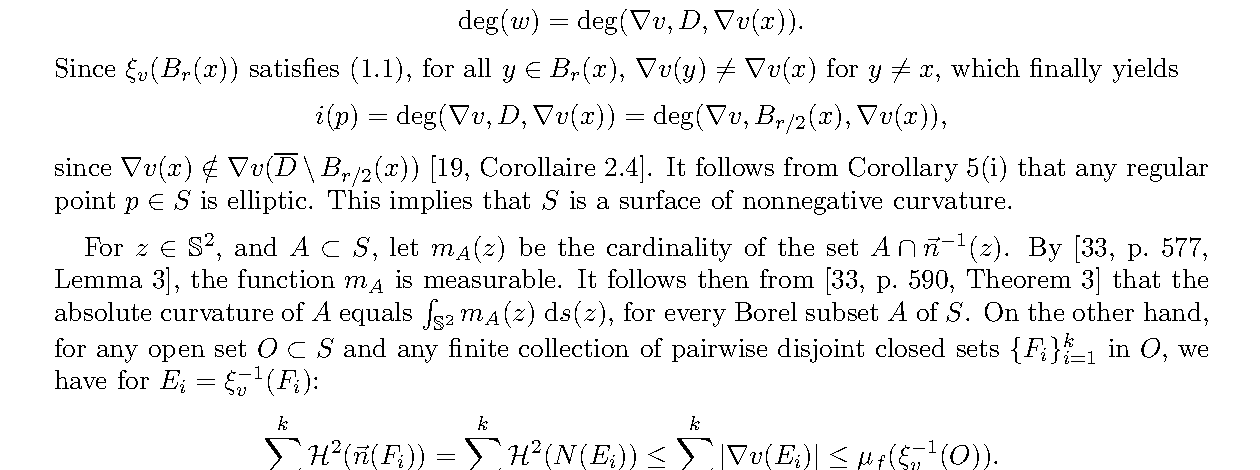
\includegraphics[width=.95\textwidth]{figures/source_elliptic_point_crop.png}
\end{center}

The other input is Ball's theorem.  Guerra and Tione state it in exactly the
needed low-regularity form: if $U$ is convex, $u\in C^1(U)$, $\nabla u$ is
locally injective, and $u_{x_0}\geq0$ near one point $x_0$, then $u$ is
strictly convex on $U$ \cite[Corollary~5.2]{GT}.  Their preceding
Theorem~5.1 proves constancy of the critical groups of all affine tilts and
gives a new proof of Ball's original result \cite{Ball}.

\begin{center}
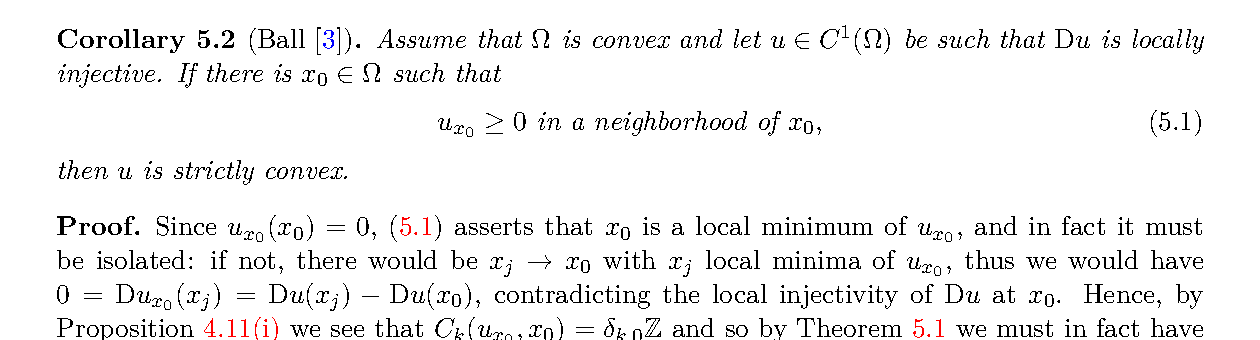
\includegraphics[width=.95\textwidth]{figures/supporting_ball_corollary_crop.png}
\end{center}

\section*{Proof of Theorem~\ref{thm:main}}

Fix $x\in\Omega$.  Choose a ball $B\Subset\Omega$ containing $x$ on which
$\nabla v$ is injective.  Every point of the graph over $B$ is regular and
hence, by Pakzad's result above, elliptic.  In particular the tangent plane
at $(x,v(x))$ meets a smaller graph neighborhood only at that point.  In
graph coordinates this says
\[
 v_x(z)\neq0\qquad(0<|z-x|<r)
\]
for some $r>0$.  A punctured planar ball is connected, so $v_x$ has one
strict sign there.  Consequently $x$ is either a strict local minimum or a
strict local maximum of $v_x$.

If it is a minimum, apply Ball's theorem to $v$ on a smaller convex ball; if
it is a maximum, apply it to $-v$.  Thus every point has a ball on which one
of $v,-v$ is strictly convex.  Opposite signs cannot occur on two
overlapping balls: on their open intersection the same function would be
both strictly convex and strictly concave.  Since a connected open subset of
$\RR^2$ is path connected, a finite chain of overlapping balls along a path
shows that one sign $\sigma$ works throughout $\Omega$.

If $\Omega$ is convex, local convexity implies convexity on all of $\Omega$
(restrict to line segments).  Equality in a convexity inequality along a
nontrivial segment would make $\sigma v$ affine on that segment, contradicting
strict convexity on a small ball about an interior point.  Hence the global
convexity is strict.

It remains to identify the measure.  Put $w=\sigma v$.  On each convex
$U\Subset\Omega$, $w$ is convex.  Mollify on a slightly larger set.  Then
$w_\varepsilon$ is smooth and convex,
\[
 \MA_{w_\varepsilon}
   =\det D^2w_\varepsilon\,dx
   =\Detw w_\varepsilon,
\]
and $w_\varepsilon\to w$ locally uniformly.  Stability of Alexandrov
measures under local uniform convergence of convex functions gives
$\MA_{w_\varepsilon}\rightharpoonup\MA_w$.  On the other hand,
\[
 \Detw w=-\tfrac12\operatorname{curl}\operatorname{curl}
       (\nabla w\otimes\nabla w)
\]
and $\nabla w_\varepsilon\otimes\nabla w_\varepsilon$ converges locally
uniformly to $\nabla w\otimes\nabla w$, so the same smooth measures converge
distributionally to $\Detw w$.  Since
$\Detw(\sigma v)=\Detw v=f$ in dimension two, uniqueness of the limit gives
$\MA_w=\mu_f$ on $U$.  Exhausting $\Omega$ by such patches completes the
proof. \qed

\section*{Provenance, search bounds, and limitation}

The packet records a direct implication of known theorems, not a newly
claimed Monge--Amp\`ere theorem.  Pakzad supplies the nonnegative-degree and
elliptic-point statement.  Ball supplies the propagation from one local
support plane to strict convexity; Guerra and Tione provide a recent,
explicit $C^1$ formulation and proof.  Guerra and Tione do not cite
arXiv:2206.09224 or state that they answer its arbitrary-domain problem, so
the link is an agent-identified literature implication rather than an
explicit later answer.

The run's cheap indexes were searched for arXiv:2206.09224, its title,
``arbitrary domain,'' ``very weak Monge--Amp\`ere,'' ``locally injective
gradient,'' and the degree/change-of-variables keywords.  A bounded
web/arXiv search added ``gradient local homeomorphism,'' ``gradient index,''
and ``strict convexity Ball,'' and found arXiv:2506.03906 and Ball's 1980
paper.  No exact published statement of Theorem~\ref{thm:main} was found.

The original problem remains open because $f\geq0$ is not known to make
$\nabla v$ locally discrete or locally injective.  The packet does not weaken
that added hypothesis.  Human review should focus on the localization of
Pakzad's elliptic-point conclusion and on the standard Alexandrov-measure
limit in the final paragraph.

\begin{thebibliography}{9}

\bibitem{Pakzad}
M.~R. Pakzad,
\emph{Convexity of weakly regular surfaces of distributional nonnegative
intrinsic curvature},
J. Funct. Anal. \textbf{287} (2024), 110539;
arXiv:2206.09224v2,
\href{https://arxiv.org/abs/2206.09224}{arXiv:2206.09224}.

\bibitem{GT}
A.~Guerra and R.~Tione,
\emph{Constancy of the index for gradient mappings},
arXiv:2506.03906v2 (2025), Theorem~5.1 and Corollary~5.2,
\href{https://arxiv.org/abs/2506.03906}{arXiv:2506.03906}.

\bibitem{Ball}
J.~M. Ball,
\emph{Strict convexity, strong ellipticity, and regularity in the calculus
of variations},
Math. Proc. Cambridge Philos. Soc. \textbf{87} (1980), 501--513.

\bibitem{Pogorelov}
A.~V. Pogorelov,
\emph{Extrinsic Geometry of Convex Surfaces},
Translations of Mathematical Monographs 35, AMS, 1973.

\bibitem{Borisenko}
A.~A. Borisenko,
\emph{Isometric immersions of space forms into Riemannian and pseudo-Riemannian
spaces of constant curvature},
Russian Math. Surveys \textbf{56} (2001), 425--497.

\end{thebibliography}

\end{document}
